\documentclass[letter, 11pt,titlepage]{article}

% Need to do some more reading: http://plain-text.co/pull-it-together.html
% Convert from LaTeX to Markdown:
% pandoc --standalone --wrap=none --base-header-level=2 -f latex -t gfm+smart+citations --filter=pandoc-citeproc --bibliography=Geopyter.bib --csl=apalike.csl -M Title="GeoPyTeR: Mashable (Geography) Teaching Resources for Python" -B header.md Geopyter.tex -o README.md

\newcommand{\gp}{\textsc{g}eo\textsc{p}y\textsc{t}e\textsc{r}~\/}
\newcommand{\eg}{e.g.~\/}
\newcommand{\ie}{i.e.~\/}
\newcommand{\pysal}{\textsc{p}y\textsc{sal}~\/}
\newcommand{\comment}[1]{\todo[inline, color=green!40]{#1}}

%% Language and font encodings
\usepackage[english]{babel}
\usepackage[utf8x]{inputenc}
\usepackage[T1]{fontenc}
\usepackage[hyphens]{url}
\usepackage{fancyvrb} % facny verbatim
\usepackage{textcomp}
\usepackage{upquote}  % Turns quotes in verbatim to straight
\usepackage{varioref} % for vpageref[above]
\usepackage{fullpage}
\usepackage{graphicx} 
\usepackage{tabularx}
\newcolumntype{s}{>{\hsize=.25\hsize \raggedright\arraybackslash}X}
\newcolumntype{b}{>{\hsize=.75\hsize}X} 	
\usepackage{booktabs}
\usepackage{wrapfig}
\usepackage[font=small,labelfont=bf]{caption}
%% Sets page size and margins
%\usepackage[letter,top=3cm,bottom=2cm,left=3cm,right=3cm,marginparwidth=1.75cm]{geometry}

%% For writing 'code' in LaTeX
\usepackage{textcomp}
\usepackage{listings}
\lstloadlanguages{Python,Perl,HTML}
\usepackage[dvipsnames]{xcolor}
\definecolor{LightGray}{gray}{0.95}
\lstset{% general command to set parameter(s)
	basicstyle=\small\ttfamily, % print whole listing small
	keywordstyle=\color{BrickRed}\bfseries,
	% underlined bold black keywords
	identifierstyle=\color{Fuchsia}, % nothing happens
	commentstyle=\color{Orange}\bfseries, % white comments
	stringstyle=\color{OliveGreen}, % typewriter type for strings
	showstringspaces=false} % no special string spaces
\lstset{frameround=tttt,backgroundcolor=\color{LightGray},framesep=8pt,rulecolor=\color{Gray}}

%% For citations
%\usepackage{natbib}
\usepackage[%
% numberedbib,
  natbibapa
]{apacite} 

%% Useful packages
\usepackage{amsmath}
\usepackage[colorinlistoftodos]{todonotes}
\usepackage[colorlinks=false, allcolors=black]{hyperref}
\def\tightlist{}

\title{Geographical Python Teaching Resources: GeoPyTeR}
\author{Jonathan Reades \and Sergio J. Rey}
%\author{}

\begin{document}
\maketitle

\begin{abstract}
Geopyter, an acronym of Geographical Python Teaching Resources, provides
a hub for the distribution of `best practice' in computational and
spatial analytic instruction; enabling instructors to quickly and
flexibly remix contributed content to suit their needs and delivery
framework; and encouraging contributors from around the world to `give
back' whether in terms of how to teach individual concepts or deliver
whole courses. As such, Geopyter is positioned at the confluence of two
powerful streams of thought in software and education: the Free and Open
Source Software (FOSS) movement in which contributors help to build
better software, usually on an unpaid basis, in return for having access
to better tools and the recognition of their peers); and the rise of
Massive Open Online Courses (MOOCs), which seek to radically expand
access to education by moving course content online and providing access
to students anywhere in the world at little or no cost. This paper sets
out in greater detail the origins and inspiration for Geopyter, the
design of the system and, through examples, the types of innovative
workflows that it enables for teachers. We believe that tools like
Geopyter, which build on open teaching practices and promote the
development of a shared understanding of what it is to \emph{be} a
computational geographer represent an opportunity to expand the impact
of this second wave of innovation in instruction while reducing the
demands placed on those actively teaching in this area.
\end{abstract}


\section{Introduction}\label{introduction}

Although \citet{Donoho2017} traces the origins of data science back to
\citeauthor{Tukey1962}'s \emph{The future of data analysis}
(\citeyear{Tukey1962}), it is only recently that this set of previously disparate practices for working with large data sets has begun to be formalised in a way that might allow it to be taught in a university context instead of acquired on the job through `learning-by-doing'. One of the most profound practical impacts of this development has been on the ways in which developers share and execute code: although systems for combining code, commentary, and results have been around for some time (\eg R-Markdown) these were intended primarily for replicating research outputs, with teaching and interaction as secondary considerations. The emergence of data science---and the overall pace of change in the tools and programming libraries that it employs---gave new impetus to the search for lightweight ways of sharing code and documentation, and an interactive browser-based platform called Jupyter \citep{kluyver16} was the result.


University educators in many disciplines are playing catch-up, but Geography---thanks to its long relationship with computation \citep{ArribasBel2018}---has been acutely aware of these developments: changes in the volume and extent of spatial data available (\eg \citealp{Graham2013,gonzalez2013big,reades2016}), and in the number and range of methods employed to identify patterns in those data (\eg \citealp{Fan2016,Naik2017,Santibanez2015,Stevens2015,ArribasBel2017}), are allowing us to tackle questions thought unanswerable just a few years ago. In academia, there has been a `turn' towards coding (\eg \citealp{Brunsdon:2020aa}), but this has not been matched by changes in our teaching practice and there is evidence of a `hollowing out' of once domain-specific skills \citep{Singleton2014,Singleton2016}: most of what used to be done with specialist Geographic Information Systems (\textsc{gis}) software can now be done using free online resources (\eg Google's Fusion Tables, MapBox, Carto, ArcOnline). However, most countries have actually seen an increase in `geospatial jobs' \citep{Solis:2020aa} indicating unmet demand for graduates who can \emph{code} using the latest (geo)algorithms and techniques. In this article we present one means of bringing the benefits of (spatial) data science-approaches to instruction using Jupyter `notebooks' for the teaching of the Python programming language and geospatial analysis.

\section{Statement of Need}

Regardless of whether this is a revolution \citep{Wyly2014,Torrens2010} or an
evolution \citep{Barnes2013,Barnes2014}, there is no question that teaching
students and researchers how to code and how to \emph{think} computationally \citep{Barba_2015_bids} presents new challenges \citep{Etherington2016,Muller2014,rey_09jgs} and that there is little in the way of a tradition of doing so to a high level within Geography (see surveys in \citealp{Bowlick2017,Bowlick2018}). Consequently, the majority of spatial data science and analytics resources used in the classroom are being developed from scratch at each institution, often by newly-appointed lecturers and assistant professors coming from the relatively small number of elite research facilities active in this domain (see discussion in \citealp{esrc2013}). Not only has this led to the duplication of effort at multiple sites, but it also has an enormous impact on the productivity of early career researchers, many of whom are in their first teaching post.

The overarching purpose of this software is therefore to address two seemingly contradictory issues: the recognition that no two instructors teach in precisely the same way, and the fact that few instructors have the luxury of both time and tenure to develop compelling new course material in splendid isolation. This is  where the Geographical Python Teaching Resource (\textsc{g}eo\textsc{p}y\textsc{t}e\textsc{r}) comes into play: although developed with geographers in mind, it provides a generic means by which instructors in any discipline can selectively incorporate and re-mix programming and conceptual content from existing Jupyter notebooks while providing their own `gloss' for this content. Our approach therefore seeks to develop a rich community of developers and teachers who work \emph{together} on new teaching materials, who make their output entirely \emph{open} to the wider community, and who \emph{support} instructors in quickly adapting existing materials to new delivery formats. It should also be noted that our tool is fully compatible with notebooks written in other languages, such as R and its powerful geospatial analytics framework (see \citealp{Bivand:2020aa} for an overview).

\section{Origins and Inspirations}\label{origins-and-inspirations}

Like many open source projects, \gp grew out of a need to scratch an itch: in our roles as teachers of (geo)computational concepts and methods we grappled on an annual basis with the demands of developing and updating instructional material with complex interdependencies. And, while the fundamental computing and analytic concepts may remain fairly stable, the field is highly-dynamic in terms of both the content (\ie what should be in the curriculum) and the code (\ie how applications should be taught). Although, in principle, there should be little interaction between curriculum and code, in practice changes to software libraries can make certain connections much harder, or much easier, to establish in the mind of the learner. For instance, until the widespread adoption of \texttt{geopandas} in Python (which itself depended on the widespread adoption of \texttt{pandas}) it was common to find that each spatial analysis library had its own data structures\footnote{A similar effect could be seen in \texttt{R} with the \texttt{tidyverse} and \texttt{sftools}.} and, consequently, students needed to be taught to work with spatial data in different ways depending on the library. Consolidation around a single approach freed up a lot of `space' in the curriculum for teaching content, not format.

In spite of this, every time a widely-used library is updated a protracted sequence of revisions ensues as teachers need to decide whether to resist making use of, or even alerting students to, the new features in order to save updating their materials, or whether to leap in enthusiastically only to struggle with conflicting dependencies and unstable feature sets. But on the basis that `many hands makes light work', we initially explored with other faculty the potential to `divide and conquer': we would each focus on different topics using the latest codebase and then combine these contributions to create a full course. Though received with some enthusiasm, this plan did not survive contact with reality: first, when actually faced with the uncertain promise of receiving a full course in return for our individual efforts, many of us felt more secure developing our own material; second, we had underestimated the value that we each attach to the ability to personalise material to our own style of teaching. Since the shared materials were being developed according to individual `style', any rationalisation or personalisation would have to be done by the instructor at a later date.

Going back to the drawing board, we looked again at our own experiences of successful programming and instructional efforts. In particular, we took note of two powerful streams of thought in software and education with which we already familiar: the importance attached by the Free and Open Source Software (\textsc{foss}) movement to both peer-recognition \citep{raymond_cathedral_1999} and distributed control; and the rise of Virtual Learning Environments (\textsc{vle}s) and Massive Open Online Courses (\textsc{mooc}s) with their use of rich, online learning experiences (\eg \citealp{Trafford2011,Cabiria2012}). Reflecting on our initial failure, we decided against trying to supply a single set of polished course materials and instead looked for a way to provide teachers with building blocks from which they could assemble an \emph{individualised} course suited to their institutional and pedagogical needs.

We drew inspiration from the original \textsc{foss} iPython project \citep{perez_2007_ipython}---expanded into the Jupyter project in 2016 \citep{kluyver16}---and its transformative impact on the sharing of integrated code, text, and multimedia resources. And we also looked to the Python Spatial Analysis Library (\textsc{p}y\textsc{sal}) project \citep{rey_19sea} in which contributors take ownership of particular application areas through managed collaboration instead of a contributory `free-for-all'. The subsequent growth of the Jupyter project has produced a rich ecosystem of tools to support the kinds of interaction needed to make this an effective teaching resource: multiuser-notebooks (\texttt{jupyterhub}), automation of grading (\texttt{nbgrader}), interactive widgets for visualisation (\texttt{ipywidgets}), and packages to facilitate manipulation of the notebook itself (\texttt{nbformat} and \texttt{notebook}).

With these criteria and resources in mind, we began looking for ways to lower the `entry costs' for faculty to both take from, and share into, a corpus of instructional material, as well as for a way to address the customisation/localisation challenge. \gp is our solution: a single, open hub of geographically-focussed teaching concepts and practical programming tasks that can be flexibly assembled into classes, or entire courses! \gp recognises that teachers need to be able to develop their own classroom `story' at their own pace (and in conformance with their institution's teaching patterns), while supporting them with a library of up-to-date materials from which they can pick and choose. So in much the same way that a computer application is compiled from the contributions of many developers, \gp allows individual classes and entire courses to be `compiled' from the contributions of many skilled teachers and developers. As such, this positions our work within contextualised programming initiatives \citep{Guzdial2010,Lukkarinen2016}, of which the CS+X approach is perhaps best-known \citep[\eg][]{Mir2017}; however, \gp represents an important advance in this area since it not only builds in context at the level of individual modules, but at the level of teaching resources as well!

Without realising it, we were plugging into a larger framework of thinking emerging from the literature on Open Educational Resources (\textsc{oer}), which began as largely `legal and economic concept' designed to support royalty and license free access to educational resources \citep{butcher2010open}. It should be clear from this definition that there is no \emph{necessary} link to \textsc{foss}, or to open and reproducible research \citep{Brunsdon:2020aa}, since a free e-book can qualify as an \textsc{oer}. However, these two areas are conceptually aligned in many ways, not least through their shared interest in the `4 Rs': reuse, redistribution, revision, and remixing \citep{Hilton2010}. Within \citeauthor{du2017}'s \citeyearpar{du2017} \textsc{oer} typology \gp is clearly `open courseware', but it is conceptually distinct from \textsc{mit}'s eponymous OpenCourseWare or Standford's Coursera since it is designed to promote what \citeauthor{Ehlers2011} calls `Open Educational Practice' \citeyearpar{Ehlers2011} in a manner not altogether dissimilar to that the Geographic Science \& Technology Body of Knowledge \citep{bok2018}.

In line with \citet{Mishra2017} and with \citeauthor{Knox2013}'s \citeyearpar{Knox2013} call for a role for pedagogy in \textsc{oer}, \gp envisions an essential role for `teachers as (co)creators': they not only have an active role in selecting components for a Session or Module, they can contribute source material as well. The educator and section editors, of which more later, may therefore also use this process to extend their own understanding in an applied workplace setting through collaboration (see \citealp{littlejohn2017} and \citealp{eraut2008} for relevant discussions). Of course, we must also recognise that under \citeauthor{Wiley2009}'s \citeyearpar{Wiley2009} \textsc{alms} typology, although \gp provides direct Access to editing tools, is Meaningfully editable, and offers Source-file access, the Level of expertise required is not insubstantial though we also expect instructors in this domain to be more comfortable than most with the process. We therefore believe that \gp is unique in incorporating the instructor's domain expertise and pedagogical strategies by design. 

\section{System Architecture}\label{system-architecture}

At least in our experience, the pace of technological and methodological change in spatial data science is such that the gap between what instructors know and what students know is substantial, and in many cases might even be growing. But the differences within individual student cohorts may be greater still, and instructors need to be able to quickly assemble and update a course that meets students where they \emph{are} rather than where the instructor or institution might \emph{wish} them to be. At the same time, there is also a strong need to support more open-ended exploration during `practicals' \citep{Unwin1980}, particularly by more advanced students who may `tune out' if progression is overly structured and rigid\ldots or just too slow to keep their attention.

The guiding insight behind \gp is that instruction in programming outside of Computer Science proceeds from fundamental units of learning typically built around \emph{computing} concepts (variables, lists/arrays, dictionaries/hashes, functions/subroutines, etc.) to fundamental units of learning built around \emph{analytic} concepts (cluster analysis, point patterns, spatial autocorrelation, etc.). These units must then be assembled in a way that speaks to the student cohort and its background; we mean this in two ways: first, that the examples used must be domain-specific in order to speak to budding geographers, political scientists, historians, etc.; and second, that it should be possible to develop courses for different types of cohorts without having to start over from scratch. In other words, how can we enable teachers to reuse many of the building blocks employed in an advanced course for Masters students in an introductory course for Undergraduates?

\subsection{Components}\label{components}

From these constraints it was clear that our system needed to support a compositional, `bottom-up' approach to instructional design. So although the development of a course or class should obviously start out with a clear set of learning aims and outcomes, at a certain point the instructor will be searching for examples and code with which to teach a particular concept: What \emph{is} a list or dictionary? What \emph{is} \emph{k}-means clustering? We settled on the term `Atoms' to refer to these basic instructional units and, much like entries in the atomic table, we felt that they could be grouped together into sets of related concepts: the fundamentals of programming, point pattern analysis, machine learning, etc.


\begin{table}[htbp]
\centering
\caption{Overview of System Components}
\label{table:1}
\begin{tabularx}{0.6\textwidth}{sb}
 \toprule
 \textbf{Concept} & \textbf{Usage} \\
 \midrule
 Atom  & A `teachable idea' combining explanation and code for a core, typically singular, concept (\eg Variables, Lists, Projections, Robust Rescaling\ldots). \\
 Sessions  & A `teachable unit' combining \textbf{multiple atoms} for delivery in a particular learning context (\eg Beginner Lab-based Course, Intermediate Flipped Module, Online Course\ldots) \\
 Modules  & A \textbf{sequence of sessions} designed to achieve one or more pedagogical objective and/or required for credit in a particular education context. \\
\bottomrule 
\end{tabularx}
\end{table}

Each Atom would employ \emph{domain-specific} illustrative examples and code so as to anchor learning in problems and applications relevant to the learner\footnote{\gp is intended for Geography and Planning students, but could quite easily be `forked' to provide a similar set of domain-specific resources for economics, sociology, or literature students.}. An Atom could start by showing how a list can be used to hold data about cities (\eg name, country, population), and a subsequent set of `cells' (the basic `unit' of Jupyter a notebook) could build on this with an an illustration of how a list-of-lists allows us to add location as a latitude and longitude coordinate pair. We will return to some of the issues that this approach raises in \nameref{sec:engagement}, but it points to the importance of ensuring a degree of consistency in how the Atoms for a set of closely-related topics fit together. 

The purpose of the bottom-up approach is that these units can then be flexibly assembled into Sessions: from the \emph{same ingredients} (\ie Atoms) the instructor could create quite different modules by organising and presenting the elements in different ways. Quite simply, we don't want to have to rewrite material for each format (\eg lecture/practical, `flipped' classroom, or distance learning), but we also need to deal with the fact that different types of scaffolding are required and that the amount of content suitable to a `class' in each of these formats might differ substantially. 

Furthermore, sessions designed for experts (\eg those pursuing continuing online education) might be able to `move' students through many more Atoms of instruction in a single Session than a similarly laid out on designed for first-time programmers in an undergraduate programme. So Sessions need to be able to \emph{incorporate} Atoms in a way that minimises the level of effort involved in finding the `best' way to, for example, explain the concept of recursion while maximising the ability of the instructor to relate this concept to the students' practical experience (\eg by providing a `context' that is anchored in a locally relevant `story' or data).

Naturally, Sessions can then be grouped into Learning Modules that offer a coherent instructional programme over a period of weeks or months. Modules represent the highest level of abstraction in the proposed system, but they are also obviously the starting point from which instructors can organise their (remixed) atomic and sessional material into something incorporating a set of learning outcomes and a package of assessment appropriate to their students. However, our design reflects the expectation that contributions to \gp at each \emph{level} of instruction might be made by \emph{different} people: a domain expert in Spatial Bayes might be the right person to develop an Atom on the concept and its application, but not the right person to develop a module tackling advanced spatial analytic concepts where this is just one approach amongst many. Similarly, given the global diversity of delivery formats, a 10-week term in Britain enables students to cover a very different `volume' of content from a 15-week American semester. \gp recognises and seeks to respond to that diversity.

\subsection{Tools}\label{tools}

So we are trying to design a system in which Sessions and Modules are \emph{composed} out of Atoms that can be, optionally, surrounded by the instructor's own `narrative'. We therefore want to produce a set of teaching materials that are highly portable, easily re-used or edited, and that enable the instructor to select only the elements from which they wish to compose their materials. As intimated above, \gp operationalises this through the Jupyter project and its ability to provide in-browser access to the Python interpreter\footnote{Other languages are also possible using different kernels; there is no reason that \gp couldn't be used to create instructional materials in these languages as well.}, and it also takes advantage of the dominance of the Git version control tool---and the GitHub service/web site---as a means of tracking authorship across edits.

In theory, thanks to the combination of Jupyter and GitHub is not even necessary
for the novice user to have Python installed on their own computer: since all
interaction with Python is via the browser, the environment could be hosted on a
server halfway round the world. In practice, however, there are few such
services and most users simply download and install a free version of Python
(\eg Anaconda) that will run on their system. In our field many people are
already using this approach: notebooks can be found covering everything from
introductory concepts \citep{millington_reades_2017_code} to advanced spatial
analysis methods \citep{darribas_gds15}, and combined for both complete courses
or workshops \citep{rey_2016_narsc}.

Jupyter notebooks are written as a mix of executable code cells and non-executable text formatted with the widely-used `markdown' syntax. Notebook structure is provided through headers in markdown cells: a `\#' pre-pended to a line of text is generally taken to be the title of the notebook; `\#\#' at the start of a line provides a second level of structure (\ie Level 2 headers); `\#\#\#' indicates Level 3 headers; etc. For our purposes, what's relevant is that these headers naturally yield a semantic hierarchy that corresponds closely to the h1\ldots{}h6 model used by the HTML markup language that lies at the heart of the World Wide Web. This hierarchy allows us to `abstract out' the problem of inferring the \emph{meaning} of cells in different sections of the notebook since the instructor does it for us through their use of headers.

\subsection{Approach}

In order to assemble Atoms into Sessions and Modules, \gp necessarily requires a compositional syntax. We've noted the conceptual mapping between markdown and \textsc{html} formatting above, but how do we select some mix of code and markdown material in one notebook to be incorporated into another? And how do we do this in a way that is both simple to express and able to resolve ambiguity? Fortunately, such a model already exists and was hinted at in Figure \ref{fig:structure}: Cascading Style Sheets (\textsc{css}) uses well-understood `selectors' to specify one or more elements on a web page to which a set of presentational styles should be applied. 

In \textsc{css} an `h1' in a style sheet indicates that all \textsc{html} Level 1 Headers (\eg \texttt{<h1>A Title</h1>}) should observe the styling rules declared immediately afterwards; while `h1.important' specifies that only a Level 1 Header of the class `important' should be selected (\eg \texttt{<h1 class="important">A Title</h1>}) and all other Level 1 headers ignored (\eg \texttt{<h1 class="unimportant">A Title</h1>}). In fact, \textsc{css} also allows for nested selectors in which `child' element(s) of a `parent' can be selected in turn. This is normally used to do things like specify mouseover behaviours for a menu: that all anchors (\ie links) that are within a division of class \texttt{menu} should act in \emph{this} way when the mouse passes over them (\eg \texttt{div.menu a.hover}). What is particularly elegant about \textsc{css} is that it provides a means for selecting multiple pieces of content in the document in one declaration (where this is desirable) \emph{and} a means for disambiguating content with the same name but in different locations within a document hierarchy (where it is not). 

Conceptually, \gp adapts this syntax to allow us to select some or all of a Jupyter notebook using the structure imparted by the instructor: all cells coming after a Level 1 Header are considered to be part of that element's semantic field until another Level 1 Header is encountered or the end of the document is encountered, whichever comes first. And a Level 2 Header coming `after' (a `child', if you prefer) a Level 1 Header is considered part of that `parent' element's semantic field, \emph{but} we can select it uniquely within the notebook using the standard \textsc{css} form of \texttt{h1.content h2.subcontent}. This is illustrated in schematic form in Figure \ref{fig:structure}, but note that the \texttt{>} is simply make clear the hierarchical relationship. With this, we have essentially repurposed \textsc{css} as a means of selecting and importing content from one notebook into another!

\begin{figure}[htbp]
  \centering
  \caption{Illustration of a single Atom's Structure}
  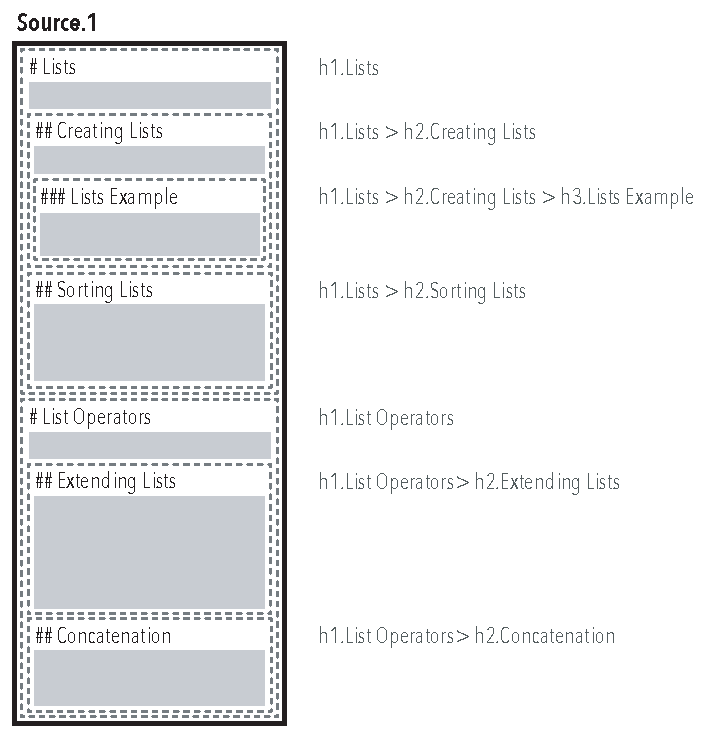
\includegraphics[width=0.5\textwidth]{Single_Document.pdf}
  \label{fig:structure}
\end{figure}

Unfortunately, the nature of Jupyter notebooks does not allow this to happen dynamically at run-time, but it does allow something similar to happen when an instructor is `compiling' new Sessional and Module content. In short, the instructor writes whatever content they wish but, using syntax similar to the examples below, wherever they want to incorporate contributed content from \gp (or elsewhere) they have only to `include' it by specifying both a source and a selection. And this approach works recursively: a notebook can include content from a notebook that itself includes content from another notebook.
\subsection{Syntax}\label{syntax}

To recap, we typically envision an Atom as a short notebook focussing on a core concept or method (\eg lists, object-oriented design, or spatial autocorrelation); some or all of each Atom can then be selected and imported into a Session, which is itself a notebook; and the sessions can then be selected and managed through a Module, which can \emph{also} be a notebook or a set of notebooks. This process is initiated by the instructor creating a blank text cell in a Jupyter notebook and writing an `include' statement. The statement should be the \emph{only} content in the cell since \gp will be replacing the cell with an unknown number of whole text and code cells from the referenced notebook.

Crucially, \texttt{include} statements can be freely intermingled with the instructor's own content (as shown in Figure \ref{fig:include}, allowing the instructor to `frame' the concepts in a way that suits their teaching style but which saves them having to reinvent the wheel for each class. A Session tackling standardisation could include elements of the relevant Atom from \gp while still allowing the instructor to interject comments, observations, questions, and additional tasks to ground the learning experience in the local context (individual, institutional, etc.). To illustrate this more clearly, an Atom on Python's approach to dealing with lists could be incorporated into a longer Session as follows:

\begin{figure}
	\centering 
	\caption{Illustrative Jupyter notebook content}
	\label{fig:include}
\begin{lstlisting}[language=HTML,frame=single]
# Session 2: Lists

Module leader: Associate Prof. X
Contact information: prof.x@foo.bar.uk
\end{lstlisting}	
\begin{lstlisting}[language=Python,frame=single]
@include {
    'nb'     = 'http://geopyter.org/atoms/fundamentals/lists.ipynb',
    'select' = 'h1.Lists'
}
\end{lstlisting}

\begin{lstlisting}[language=HTML,frame=single]
## All Done?

For next week please read the following: ...
\end{lstlisting}

\end{figure}

Here, \texttt{nb} is a path---local or remote---to a valid Jupyter notebook from which the instructor wants to import content. The \texttt{select} parameter specifies a selector for which the \gp tool will search within the source notebook. All content from that point onwards \emph{up to the next selector at the same level} will the then be copied into the compiled notebook. In the example above, if there were a following \texttt{h1} covering, for example, `List Operators' then this would \emph{not} be included because, from a structural standpoint, it is at the same level in the hierarchy as `Lists' but has \emph{not} been selected. Furthermore, any \texttt{h2} or \texttt{h3} subsections within the `Lists' section \emph{would} be included since they are presumed to be providing pedagogical and logical structure to the Lists section and so should be carried over.

Clearly, an instructor might want to import only part of of a section, or to suppress a subsection falling in the middle of a larger resource. In anticipation of this need more complex `include' statements with no equivalent in \textsc{css} are also possible:
\begin{Verbatim}[fontsize=\small]
@include {
    'resource' = 'http://geopyter.org/atoms/fundamentals/lists.ipynb',
    'select' = 'h1.Lists -h3.Lists Example; h1.List Operators -h2.Concatenation'
}
\end{Verbatim}
In this second example, two Level 1 section are imported at the same time and a Level 3 subsection from \emph{within} each of those sections is suppressed using the `-' syntax to indicate that the section should be removed. We diverged from the \textsc{css} standard since that selectors are not separated with commas: we wanted to allow for this punctuation to be part of a section heading and felt that semi-colons are rather more rare in that context. An additional point of difference from true \textsc{css} is that we allow spaces in the `selector' because we felt that asking teachers to translate between a natural language header (``List Operators'') and what \textsc{css} would consider a safe header (``List\_Operators'') would detract from ease-of-use.

\subsection{Putting it All Together}

Jupyter notebooks use a format called JavaScript Object Notation (\textsc{json}) that is not particularly easy for most humans to read, but as it is nonetheless highly-structured we can interact with it programmatically. The extensible nature of the \textsc{json} format also allows us to read and write both data and metadata not only to each notebook, but also to each and every cell in a notebook. Since metadata that is not understood by Jupyter is simply ignored, we can add our own fields to provide useful information related to instruction such as who should be given credit for contributing and any dependencies or requirements for installed libraries.

Taken together, this provides the foundation for remixing/mashing up content while still enabling to add an institutional or course-specific gloss wherever necessary. Each notebook might start with the instructor's contact information or by providing instructions for setting up the computing environment, but then make use of material developed by others for actual instruction. This process may seem quite abstract---and probably quite convoluted as well---but an illustration (Figure \ref{fig:compiling} \vpageref[below]{fig:compiling}) may help to clarify why this process is so useful.

\begin{figure}[hbtp]
  \centering
  \caption{Illustration of \gp Notebook `Compilation' Process}
  \label{fig:compiling}
  \includegraphics[width=\textwidth, angle=0]{Multiple_Documents.pdf}
\end{figure}

\section{Use Cases}\label{uses}

To illustrate how this approach offers a substantively new way to think about teaching programming material more generally, we here present two schematic use-cases: an online module of eight sessions, and an in-person module lasting one semester. It's important to stress that we envision \emph{both} of these modules being built out of the same Atoms and that, because they are drawing from version-controlled source code, the content can be fixed on a particular release (\ie version).

\subsection{Distance Learning Module}\label{an-online-module}

There has been increasing interest at universities in Massive Open Online Courses, or \textsc{mooc}s, as vehicles for expanding access to higher education through online delivery. For managers in Higher Education (\textsc{he}), the \textsc{mooc} promises both enhanced revenue and enhanced access to underserved groups. Our own experience suggests substantial student interest in `computational social science' \citep{Lazer2009}, with international students being the most keen on such modules as they are seen to provide marketable skills (programming) for graduates from a discipline (geography) with generally high employment rates (see: \citeauthor{rgs2017} \citeyear{rgs2017}).

Associate Professor X wishes to offer a \emph{Foundations of Spatial Data Science} module to second year undergraduates, but anticipates high demand exceeding her capacity to teach in  a computer cluster and high attrition since many students will decide that programming is `not for them'. Consequently, the decision is made to offer this module on a distance-learning basis with pre-recorded video content and other rich media to support student learning. However, the `remote desktop' environment that will support this module is only updated every 18 months, often in the middle of term.

\gp significantly reduces the overhead of several of these stages: rather than focussing on tasks such as how to explain or illustrate a particular concept, the instructor can focus on developing the multimedia content. The similarity between learning to code and learning a language is noted, and each `lesson' is designed to be completed in under an hour so that students can proceed at their own pace without being overwhelmed. As well, using Git tags Prof. X can `fix' the version of the code and explanations used to one that is appropriate to the computing environment while continuing to update her teaching materials.

\subsection{In-Class Delivery}\label{in-class-delivery}

Associate Professor X \emph{also} teaches a module for Masters students that follows the more traditional lecture+practical format. Although these students are also new to programming, they have already completed a required \textsc{gis} module. Here, \gp could be employed differently: since the instructor is able to interactively provide the `frame' or `scaffold' (see relevant discussion of `hypermedia' in \citealp{Azevedo2008}) upon which the learning is built, there is less need for a narrative around each task or weekly session. 

The instructor might therefore simply import the same group of Atoms as above,
but use a Session and Module template that leaves out the rich media and more
detailed explanations since these will be discussed in-class with the students.
The Sessions then wrap up with an additional mini-project or mini-assessment
that requires the students to translate the concepts into a new problem domain
or investigate the process in more detail: ``we've seen how we can use
\texttt{pandas} and \texttt{bokeh} to explore and compare the distribution of
demographic groups in London, here's a link to equivalent open data for Phoenix,
Arizona\ldots{}''.\footnote{Interactive examples that demonstrate these use
  cases are available on-line at \url{https://mybinder.org/v2/gh/pysal/geopyter/master}.}

In addition, since students are working on their own machines, the instructor can update to the latest-and-greatest much more rapidly. To enable Professor X to manage these competing requirements, we make use of Git and the GitHub web platform not only to monitor, approve, and roll back alterations to any submitted revisions, but also to provide release `tags' to which an instructor can bind a particular instance of a Session or Module. This `fixes' their course to a particular version of an Atom such that development of the Atom by others can continue without the instructor having to worry that the explanation or code upon which they rely will suddenly change! 

\section{Engagement}\label{sec:engagement}

In effect, in both of the example use cases the role of the instructor is to provide an integrative narrative that guides the students and contextualises their choice of components. We think that this has the potential to free up instructors to focus on where they can most effectively `add value'; not in developing yet \emph{another} way to show how a list or dictionary works, but in explaining why they matter to a geography, political science, or literature major (see \citealp{Bort2015} for an application in literature).

And because it builds on \textsc{foss} approaches to software development, we expect \gp to benefit from network effects: the more people use it, the more useful it becomes, and the more people use it. The open source, peer-generated approach is also, however, likely to present something of a challenge over time: as more people seek both to use and to contribute to \gp we would expect to see the emergence and use of divergent norms, examples, and data across Atoms, Sessions, and Modules. Although the emergence of difference styles of coding is actually quite natural in programming and could be seen as a benefit to students in terms of teaching them about this aspect of programming, it also the case that \gp could become a victim its own success if it ceases to be coherent.

\subsection{Coordination}


Here we believe that the \pysal project offers a useful template. Although \pysal is a \textsc{foss} project, it is \emph{not} a free-for-all: domain specialists tend to gravitate towards those parts of the project to which they have the most to contribute and, over time, those who coordinate and enable the most substantive contributions to the codebase in terms of features and performance are `invited' to help manage individual components of the tool (\eg \texttt{lib}, \texttt{model}, \texttt{explore}, \texttt{viz}). Overall coherence is maintained via regular calls and online discussion boards, as well as a synchronised release schedule so that changes can be coordinated, tested, and knock-on effects resolved.

\begin{table}[hbtp]
\centering
\caption{Indicative Groups of Atoms}
\label{table:2}
\begin{tabularx}{0.6\textwidth}{sb}
 \toprule
 \textbf{Atomic Group} & \textbf{Indicative Content} \\
 \midrule
	\texttt{auto} & Approaches to spatial autocorrelation analysis. \\
	\texttt{context} & Why learn to program? Example applications. Interviews. \\
	\texttt{networks} & Working with network data and costs. \\ 
	\texttt{describe} & Simple descriptive statistics.  \\
	\texttt{statistics} & More advanced methods of comparing data. \\
	\texttt{clustering} & Non-spatial and spatial clustering analysis. \\
	\texttt{foundations} & Foundations of programming and Computer Science. \\
	\texttt{os} & Basic aspects of interacting with Operating Systems programmatically. \\
	\texttt{viz} & Visualising data and making maps. \\
	\texttt{ml} & Approaches to Machine Learning in a spatial context. \\ 
	\texttt{points} & Point pattern generation and analysis. \\ 
	\texttt{zones} & Zonal statistics and relationship. \\
	\texttt{models} & From regression to \textsc{gwr}. \\
\bottomrule 
\end{tabularx}
\end{table}	

In general, we would expect to see a relatively small number of committed educators and developers creating and maintaining groups of Atoms that align with their areas of expertise, interests, and teaching responsibilities. However, unlike a traditional software project there is an important role here for \emph{teachers}, not just developers. We think that this represents a really exciting opportunity for innovative new approaches to rise to the surface. There may be only a few who can write the Python code to conduct a Geographically-Weighted Regression analysis, but it will be interesting to see how many creative, insightful ways there are to explain it! 

So although we also expect interested educators to begin almost immediately picking holes in the organisational structure proposed in Table \ref{table:2}, some kind of starting point is needed. Moreover, as we've mentioned elsewhere, in the event of serious disagreement other instructors are free `fork' the repository and begin changing material as they see fit. Indeed, there is nothing to prevent \gp Sessions and Modules drawing on content spread across multiple repositories following different organisational and developmental strategies: all that's need is a \textsc{url}!

The educational focus of \gp implies that it may well be the most committed teachers who end up as `section editors' who coordinate and review contributions. The editorial approach also aligns with the obvious benefits of grouping sets of Atoms together into basic sections such as \texttt{foundations} (the basics of variables and data structures); \texttt{describe} (describing data); etc. The section editor ensures that examples, style, and other features are consistent across individual Atoms to make it easy to generate a set of Sessions introducing the Unix file system or Local Indicators of Spatial Autocorrelation.

\gp therefore seeks to balance the benefits of code-sharing with those of local expertise: the instructor is free to write their own exegesis, if you will, of the code and its relevance to a particular Session or Module, but the burden of developing a cogent, domain-specific demonstration can be shared with others and compelling examples more widely adopted without the effort of reinventing the wheel. Where irreconcilable differences arise between pedagogical approaches or models, then we might expect to see small groups of collaborators `fork' the codebase and offer their own models; this is, of course, a valid approach with open source code and one from which all instructors can ultimately benefit!

\subsection{Credit}

The use of Git/GitHub also gives us access to contributor information in the `commit' (\ie editing) logs that we can propagate into notebooks so that all contributors are recognised in the final output. Although the open nature of the project means that we cannot strictly enforce attribution, \gp seeks to make this the easier to do `by default' through the insertion of metadata into the compiled notebook which is then used to append a list of contributors to the end of each notebook, along with any other relevant acknowledgments or copyright notices.

To facilitate re-use while protecting contributions from unacknowledged exploitation textual content in \gp is covered by a Creative Commons license; however, to deal with the fact that \gp relies extensively on open source contributions which are incompatible with some \textsc{cc} licenses \citep[see discussion in][]{osswatch2013}, code blocks are licensed under the \textsc{mit} license. The manner in which contributions from authors at different institutions can be combined also `pollutes' the materials in ways that inhibit institutional assertions of ownership over \gp content.

\gp also recognises the reality of the need for peer and professional recognition by incorporating attribution mechanisms directly into the compilation process. Digital Object Identifiers (\textsc{doi}s) can be created and curated by the `section editors', but authorship of \gp components---be they Atoms, Sessions or Modules---provides the contributors with peer-evaluated, impactful materials to add to promotion applications. Our intention is that both users and institutions come to better-understand the extent to which open educational resources can be a \emph{joint} project relying on the contributions of many teachers and developers.

\section{Limitations}\label{limitations}

As we noted above in connection with Table \ref{table:2}, it is rather unlikely that our first attempt to divide up the entire field into discrete units of instruction will be entirely successful. We would also expect to draw on reference documents such as the \emph{Body of Knowledge} \citep{bok2018} and \emph{Subject Benchmark Statement} \citep{QAA2014} for the `why' and `what' of instruction, leaving \gp to deal with the `how'. Moreover, the open, contributory nature of the project positions us to build \gp on top of the shared understanding of many specialists with a range of ideas about how to break apart, and put back together, the constituent elements of our domain's  knowledge in ways that speak to different types of students.

For the time being we have also deliberately hobbled \gp in one important way: an \texttt{include} command must be in a cell that does not contain any other text or code. This was done primarily for simplicity: it's a lot easier to look for whole (text) cells that match a target pattern than to have to try to parse long blocks of text or code on the off-chance that an \texttt{include} might be found; it also avoids any ambiguity as to whether the \texttt{include} is a \gp or `native' command. Not coincidentally, it is also a good deal easier to replace an entire cell (the one containing an \texttt{include}) with one or more entire cells, than to try to work out if a cell needs to be `closed out' first.

\section{Conclusion \& Future Directions}\label{future}

From practical experience, conference presentations, and code we tend to already know who is a good \emph{programmer} or \emph{theorist}, \gp provides a mechanism for discovering who is a good \emph{teacher}. Sometimes these abilities may reside in the same person, but more often we expect that they will not: the strongest developers tend to be people who have been practicing software development for many years and, consequently, may have difficulty communicating their ideas to beginner- or intermediate-level students or teachers (see: \citealp{Chapman:2010aa})! For this reason we see the broad-based community-of-practice aspect of \gp as integral at all stages of the project: system enhancement, content development, expanding coverage, and instructional design.

Consequently, \gp has a lot in common---both philosophically and practically---with the Software Carpentry movement \citep{SCF2016}, and although we seek to tackle a slightly narrower set of issues with a more re-usable set of resources, we can take both inspiration and warning from their experience. The benefit, we think, is that while it is possible to design Sessions and Modules that follow the popular `bootcamp' approach to instruction (though see critique in \citealp{Feldon2017}), we want to enable the \emph{same} content to be employed in a carpentry format as well as a `normal' classroom or \textsc{mooc} as required\ldots Or even to enable the instructor to mash all of those formats together such that they use a `bootcamp' format for the introduction to Unix and the command line, an online-formatted resource for foundational concepts in computer science, and a traditional course format for the (geo)data analysis instruction. All pulled from the same set of source Atoms!

Ultimately, although \gp was developed with teaching needs in mind there is, of course, no reason why it couldn't be put to other uses: in combination with with \texttt{nteract} (\url{https://github.com/nteract/nteract}) it would allow developers or researchers to build fully-fledged applications as scripts assembled from a collection of notebooks; or as an addition to Netflix's notebook ecology to allow for enhanced resource-sharing and standardisation during the development phase before features and interfaces are `fixed' as libraries \citep{Ufford2018}. Nonetheless, our focus for the time being remains the cohort of university teachers at all levels tasked with introducing programming material to their students and wondering where to begin. We hope that \gp makes a valuable contribution to this application domain and look forward to working with others to roll out a rich, reusable teaching framework.

\section{Supplemental}

Demonstration notebooks can be found in the `sessions' directory of the \gp project on GitHub: \href{https://github.com/pysal/geopyter/tree/master/sessions}{github.com/pysal/geopyter/tree/master/sessions}.

\bibliographystyle{apacite}
\bibliography{Geopyter.bib}

\end{document}
